\documentclass[xetex,mathserif,serif]{beamer}
\usepackage{polyglossia}
\setdefaultlanguage[babelshorthands=true]{russian}
\usepackage{minted}
\usepackage{tabu}

\useoutertheme{infolines}

\usepackage{fontspec}
\setmainfont{FreeSans}
\newfontfamily{\russianfonttt}{FreeSans}

\usepackage{textpos}
\setlength{\TPHorizModule}{1cm}
\setlength{\TPVertModule}{1cm}

\setbeamertemplate{blocks}[rounded][shadow=false]

\setbeamercolor*{block title alerted}{fg=red!50!black,bg=red!20}
\setbeamercolor*{block body alerted}{fg=black,bg=red!10}

\tabulinesep=1.2mm

\title[Декомпозиция, ООП]{Лекция 2: Декомпозиция, объектно-ориентированное проектирование}
\author[Юрий Литвинов]{Юрий Литвинов\\\small{\textcolor{gray}{y.litvinov@spbu.ru}}}
\date{25.02.2022}

\newcommand{\todo}[1] {
    \begin{center}\textcolor{red}{TODO: #1}\end{center}
}

\newcommand{\DownArrow} {
    \hspace{2cm}\begin{LARGE}$\downarrow$\end{LARGE}
}

\newcommand{\attribution}[1] {
    \begin{flushright}\begin{scriptsize}\textcolor{gray}{\textcopyright\, #1}\end{scriptsize}\end{flushright}
}

\begin{document}

    \frame{\titlepage}

    \section{Декомпозиция и модульность}

    \begin{frame}
        \frametitle{Сложность}
        \begin{itemize}
            \item \textbf{Существенная сложность} (essential complexity) --- сложность, присущая решаемой проблеме; ею можно управлять, но от неё нельзя избавиться
            \item \textbf{Случайная сложность} (accidental complexity) --- сложность, привнесённая способом решения проблемы
        \end{itemize}
        \vskip 0.5cm
        \begin{center}
            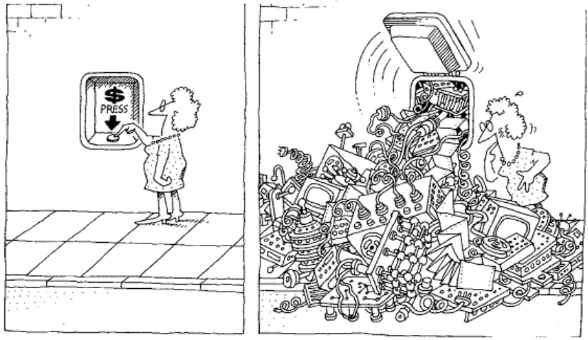
\includegraphics[width=0.5\textwidth]{complexityHiding.png}
        \end{center}
        \attribution{G. Booch, ``Object-oriented analysis and design''}
    \end{frame}

    \begin{frame}
        \frametitle{Свойства сложных систем}
        \begin{itemize}
            \item Иерархичность --- свойство системы состоять из иерархии подсистем или компонентов
            \begin{itemize}
                \item Декомпозиция
            \end{itemize}
            \item Наличие относительно небольшого количества видов компонентов, экземпляры которых сложно связаны друг с другом
            \begin{itemize}
                \item Выделение общих свойств компонентов, абстрагирование
            \end{itemize}
            \item Сложная система, как правило, является результатом эволюции простой системы
            \item Сложность вполне может превосходить человеческие интеллектуальные возможности
        \end{itemize}
    \end{frame}

    \begin{frame}
        \frametitle{Подходы к декомпозиции}
        \begin{itemize}
            \item Восходящее проектирование
            \begin{itemize}
                \item Сначала создаём ``кирпичики'', потом собираем из них всё более сложные системы
            \end{itemize}
            \item Нисходящее проектирование
            \begin{itemize}
                \item Постепенная реализация модулей
                \item Строгое задание интерфейсов
                \item Активное использование ``заглушек''
                \item Модули
                \begin{itemize}
                    \item Четкая декомпозиция
                    \item Минимизация
                    \item Один модуль --- одна функциональность
                    \item Отсутствие побочных эффектов
                    \item Независимость от других модулей
                    \item Принцип сокрытия данных
                \end{itemize}
            \end{itemize}
        \end{itemize}
    \end{frame}
    
    \begin{frame}
        \frametitle{Модульность}
        \begin{itemize}
            \item Разделение системы на компоненты
            \item Потенциально позволяет создавать сколь угодно сложные системы
            \item Строгое определение контрактов позволяет разрабатывать независимо
            \item Необходим баланс между количеством и размером модулей
        \end{itemize}
        \vskip 1cm
        \begin{center}
            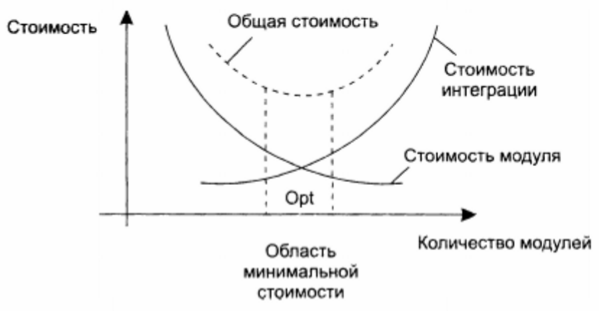
\includegraphics[width=0.5\textwidth]{modulesCost.png}
        \end{center}
    \end{frame}

    \begin{frame}
        \frametitle{Сопряжение и связность}
        \begin{itemize}
            \item \textbf{Сопряжение (Coupling)} --- мера того, насколько взаимозависимы разные модули в программе
            \item \textbf{Связность (Cohesion)} --- степень, в которой задачи, выполняемые одним модулем, связаны друг с другом
            \item Цель: слабое сопряжение и сильная связность
        \end{itemize}
    \end{frame}

    \section{Некоторые принципы ОО-проектирования}

    \begin{frame}
        \frametitle{Объекты}
        \begin{itemize}
            \item Objects may contain data, in the form of fields, often known as attributes; and code, in the form of procedures, often known as methods --- \textbf{\href{https://en.wikipedia.org/wiki/Object-oriented\_programming}{Wikipedia}}
            \item An object stores its state in fields and exposes its behavior through methods --- \textbf{\href{https://docs.oracle.com/javase/tutorial/java/concepts/object.html}{Oracle}}
            \item Each object looks quite a bit like a little computer --- it has a state, and it has operations that you can ask it to perform --- \textbf{\href{http://amzn.to/1PBmQpm}{Thinking in Java}}
            \item An object is some memory that holds a value of some type --- \textbf{\href{http://amzn.to/1XyGCtk}{The C++ Programming Language}}
            \item An object is the equivalent of the quanta from which the universe is constructed --- \textbf{\href{http://amzn.to/266oJr4}{Object Thinking}}
        \end{itemize}
    \end{frame}

    \begin{frame}
        \frametitle{Объекты}
        \begin{itemize}
            \item Имеют
            \begin{itemize}
                \item Состояние
                \begin{itemize}
                    \item Инвариант
                \end{itemize}
                \item Поведение
                \item Идентичность
            \end{itemize}
            \item Взаимодействуют через посылку и приём сообщений
            \begin{itemize}
                \item Объект вправе сам решить, как обработать вызов метода (\textbf{полиморфизм})
                \item Могут существовать в разных потоках
            \end{itemize}
            \item Как правило, являются экземплярами \textbf{классов}
        \end{itemize}
    \end{frame}

    \begin{frame}
        \frametitle{Абстракция}
        \textbf{Абстракция} выделяет существенные характеристики объекта, отличающие его от остальных объектов, с точки зрения наблюдателя
        \vskip 1cm
        \begin{center}
            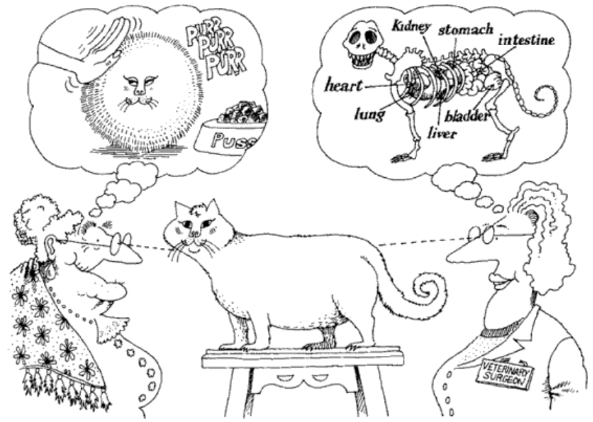
\includegraphics[width=0.45\textwidth]{abstraction.png}
        \end{center}
        \attribution{G. Booch, ``Object-oriented analysis and design''}
    \end{frame}

    \begin{frame}
        \frametitle{Инкапсуляция}
        \textbf{Инкапсуляция} разделяет интерфейс (\textbf{контракты}) абстракции и её реализацию

        Инкапсуляция защищает \textbf{инварианты} абстракции
        \vskip 1cm
        \begin{center}
            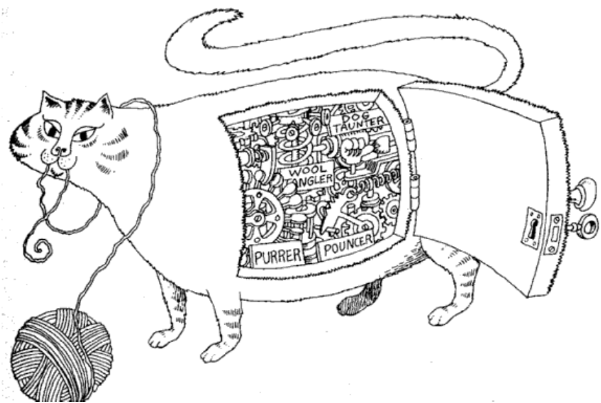
\includegraphics[width=0.45\textwidth]{incapsulation.png}
        \end{center}
        \attribution{G. Booch, ``Object-oriented analysis and design''}
    \end{frame}

    \begin{frame}
        \frametitle{Наследование и композиция}
        \begin{itemize}
            \item \textbf{Наследование}
            \begin{itemize}
                \item Отношение ``Является'' (is-a)
                \item Способ абстрагирования и классификации
                \item Средство обеспечения полиморфизма
            \end{itemize}
            \item \textbf{Композиция}
            \begin{itemize}
                \item Отношение ``Имеет'' (has-a)
                \item Способ создания динамических связей
                \item Средство обеспечения делегирования
            \end{itemize}
            \item Более-менее взаимозаменяемы
            \begin{itemize}
                \item Объект-потомок на самом деле включает в себя объект-предок
                \item Композиция обычно предпочтительнее
            \end{itemize}
        \end{itemize}
    \end{frame}

    \begin{frame}
        \frametitle{Определение объектов реального мира}
        \framesubtitle{Объектная модель предметной области}
        \begin{itemize}
            \item Определение объектов и их атрибутов
            \item Определение действий, которые могут быть выполнены над каждым объектом (назначение ответственности)
            \item Определение связей между объектами
            \item Определение интерфейса каждого объекта
        \end{itemize}
        \begin{center}
            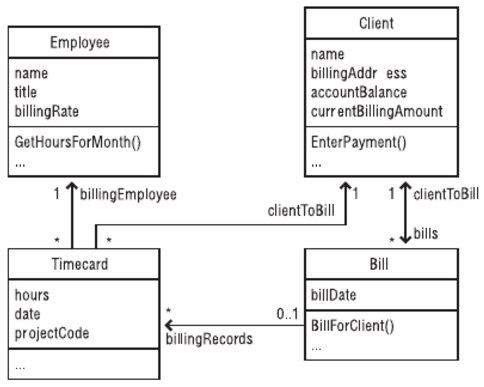
\includegraphics[width=0.35\textwidth]{billDomainModel.png}
        \end{center}
    \end{frame}

    \begin{frame}
        \frametitle{Изоляция сложности}
        \begin{columns}
            \begin{column}{0.6\textwidth}
                \begin{itemize}
                    \item Сложные алгоритмы могут быть инкапсулированы
                    \item Сложные структуры данных --- тоже
                    \item И даже сложные подсистемы
                    \item Надо внимательно следить за интерфейсами
                \end{itemize}
            \end{column}
            \begin{column}{0.4\textwidth}
                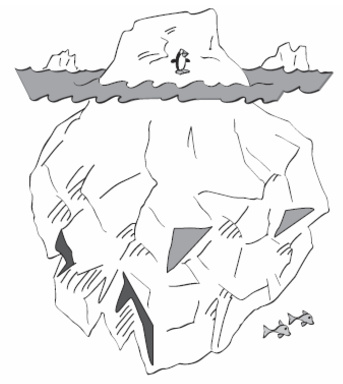
\includegraphics[width=0.7\textwidth]{complexity.png}
            \end{column}
        \end{columns}
    \end{frame}

    \begin{frame}
        \frametitle{Изоляция возможных изменений}
        \begin{itemize}
            \item Потенциальные изменения могут быть инкапсулированы
            \item Источники изменений
            \begin{itemize}
                \item Бизнес-правила
                \item Зависимости от оборудования и операционной системы
                \item Ввод-вывод
                \item Нестандартные возможности языка
                \item Сложные аспекты проектирования и конструирования
                \item Третьесторонние компоненты
                \item ...
            \end{itemize}
        \end{itemize}
    \end{frame}

    \begin{frame}
        \frametitle{Изоляция служебной функциональности}
        \begin{itemize}
            \item Служебная функциональность может быть инкапсулирована
            \begin{itemize}
                \item Репозитории
                \item Фабрики
                \item Диспетчеры, медиаторы
                \item Статические классы (\textit{Сервисы})
                \item ...
            \end{itemize}
        \end{itemize}
    \end{frame}

    \section{Принципы SOLID}
    
    \begin{frame}
        \frametitle{Принципы SOLID}
        \begin{itemize}
            \item Single responsibility principle
            \item Open/closed principle
            \item Liskov substitution principle
            \item Interface segregation principle
            \item Dependency inversion principle
        \end{itemize}
    \end{frame}

    \begin{frame}
        \frametitle{Single responsibility principle}
        \begin{itemize}
            \item Каждый объект должен иметь одну обязанность
            \item Эта обязанность должна быть полностью инкапсулирована в объект
        \end{itemize}
        \begin{flushright}
            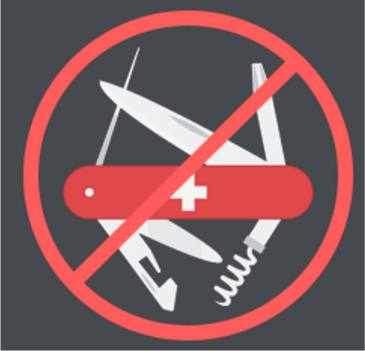
\includegraphics[width=0.25\textwidth]{singleResponsibility.png}
        \end{flushright}
    \end{frame}

    \begin{frame}
        \frametitle{Open/closed principle}
        \begin{itemize}
            \item Программные сущности (классы, модули, функции и т. п.) должны быть открыты для расширения, но закрыты для изменения
            \begin{itemize}
                \item Переиспользование через наследование
                \item Неизменные интерфейсы
            \end{itemize}
        \end{itemize}
        \begin{flushright}
            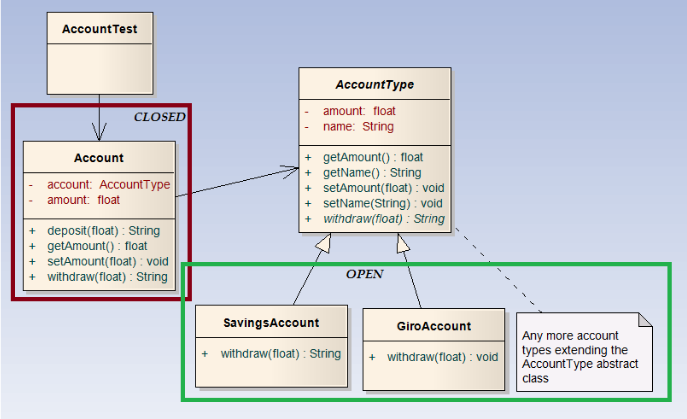
\includegraphics[width=0.5\textwidth]{openClosedPrinciple.png}
        \end{flushright}
    \end{frame}

    \begin{frame}
        \frametitle{Liskov substitution principle}
        \begin{itemize}
            \item Функции, которые используют базовый тип, должны иметь возможность использовать подтипы базового типа, не зная об этом
        \end{itemize}
        \begin{flushright}
            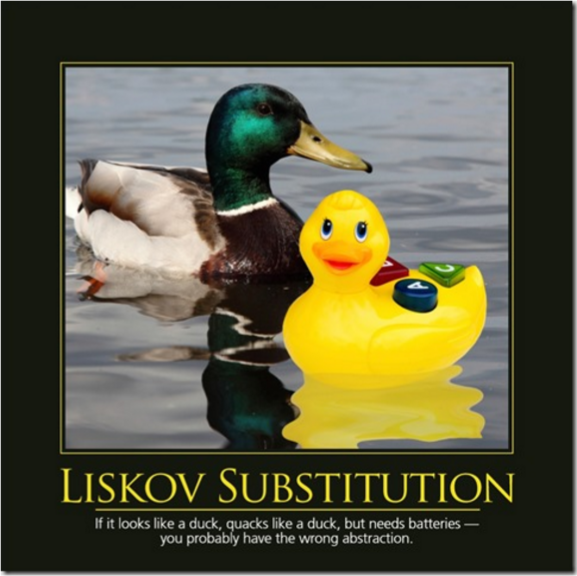
\includegraphics[width=0.4\textwidth]{liskovSubstitutionPrinciple.png}
        \end{flushright}
    \end{frame}

    \begin{frame}
        \frametitle{Interface segregation principle}
        \begin{itemize}
            \item Клиенты не должны зависеть от методов, которые они не используют
            \begin{itemize}
                \item Слишком ``толстые'' интерфейсы необходимо разделять на более мелкие и специфические
            \end{itemize}
        \end{itemize}
        \begin{flushright}
            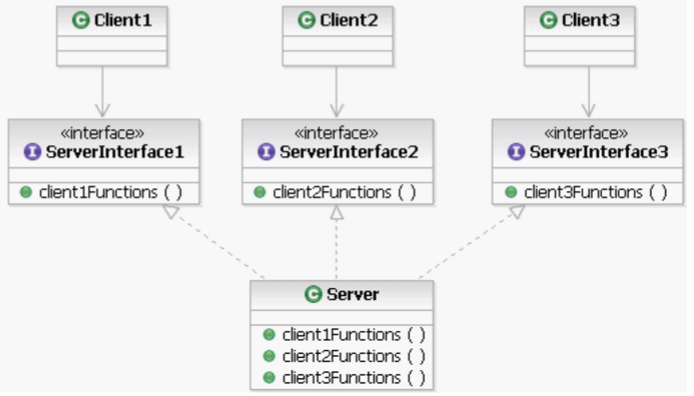
\includegraphics[width=0.5\textwidth]{interfaceSegregationPrinciple.png}
        \end{flushright}
    \end{frame}

    \begin{frame}
        \frametitle{Dependency inversion principle}
        \begin{itemize}
            \item Модули верхних уровней не должны зависеть от модулей нижних уровней. Оба типа модулей должны зависеть от абстракций
            \item Абстракции не должны зависеть от деталей. Детали должны зависеть от абстракций
        \end{itemize}
        \begin{flushright}
            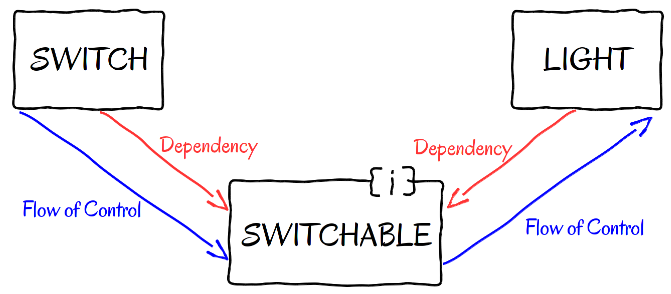
\includegraphics[width=0.5\textwidth]{dependencyInversionPrinciple.png}
        \end{flushright}
    \end{frame}

    \section{Некоторые принципы хорошего кода}

    \begin{frame}
        \frametitle{Закон Деметры}
        \begin{itemize}
            \item ``Не разговаривай с незнакомцами!''
            \item Объект A не должен иметь возможность получить непосредственный доступ к объекту C, если у объекта A есть доступ к объекту B, и у объекта B есть доступ к объекту C
            \begin{itemize}
                \item \mintinline{java}|book.pages.last.text|
                \item \mintinline{java}|book.pages().last().text()|
                \item \mintinline{java}|book.lastPageText()|
            \end{itemize}
            \item Иногда называют ``Крушение поезда''
        \end{itemize}
        \begin{flushright}
            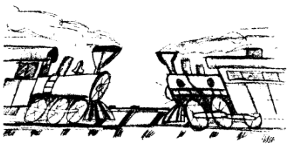
\includegraphics[width=0.35\textwidth]{trains.png}
        \end{flushright}
        \vspace{-0.8cm}
        \attribution{Р. Мартин, ``Чистый код''}
    \end{frame}

    \begin{frame}
        \frametitle{Абстрактные типы данных}
        \begin{itemize}
            \item \mintinline{java}|currentFont.size = 16| --- плохо
            \item \mintinline{java}|currentFont.size = PointsToPixels(12)| --- чуть лучше
            \item \mintinline{java}|currentFont.sizeInPixels = PointsToPixels(12)| --- ещё чуть лучше
            \item \mintinline{java}|currentFont.setSizeInPoints(sizeInPoints)| \newline
                    \mintinline{java}|currentFont.setSizeInPixels(sizeInPixels)| --- совсем хорошо
        \end{itemize}
    \end{frame}

    \begin{frame}[fragile]
        \frametitle{Пример плохой абстракции}
        \begin{minted}{java}
public class Program {
    public void initializeCommandStack() { ... }
    public void pushCommand(Command command) { ... }
    public Command popCommand() { ... }
    public void shutdownCommandStack() { ... }
    public void initializeReportFormatting() { ... }
    public void formatReport(Report report) { ... }
    public void printReport(Report report) { ... }
    public void initializeGlobalData() { ... }
    public void shutdownGlobalData() { ... }
}
        \end{minted}
\end{frame}

    \begin{frame}[fragile]
        \frametitle{Пример хорошей абстракции}
        \begin{footnotesize}
            \begin{minted}{java}
public class Employee {
    public Employee(
            FullName name,
            String address,
            String workPhone,
            String homePhone,
            TaxId taxIdNumber,
            JobClassification jobClass
    ) { ... }

    public FullName getName() { ... }
    public String getAddress() { ... }
    public String getWorkPhone() { ... }
    public String getHomePhone() { ... }
    public TaxId getTaxIdNumber() { ... }
    public JobClassification getJobClassification() { ... }
}
            \end{minted}
        \end{footnotesize}
    \end{frame}

    \begin{frame}[fragile]
        \frametitle{Ещё один пример абстракции}
        \begin{columns}
            \begin{column}{0.32\textwidth}
                \begin{minted}{java}
public class Point {
    public double x;
    public double y;
}
                \end{minted}
            \end{column}
            \begin{column}{0.05\textwidth}
                vs
            \end{column}
            \begin{column}{0.6\textwidth}
                \begin{minted}{java}
public interface Point {
    double getX();
    double getY();
    void setCartesian(double x, double y);
    double getR();
    double getTheta();
    void setPolar(double r, double theta);
}
                \end{minted}
            \end{column}
        \end{columns}
    \end{frame}

    \begin{frame}[fragile]
        \frametitle{Уровень абстракции (плохо)}
        \begin{minted}{java}
public class EmployeeRoster implements MyList<Employee> {
    public void addEmployee(Employee employee) { ... }
    public void removeEmployee(Employee employee) { ... }
    public Employee nextItemInList() { ... }
    public Employee firstItem() { ... }
    public Employee lastItem() { ... }
}
        \end{minted}
    \end{frame}

    \begin{frame}[fragile]
        \frametitle{Уровень абстракции (хорошо)}
        \begin{minted}{java}
public class EmployeeRoster {
    public void addEmployee(Employee employee) { ... }
    public void removeEmployee(Employee employee) { ... }
    public Employee nextEmployee() { ... }
    public Employee firstEmployee() { ... }
    public Employee lastEmployee() { ... }
}
        \end{minted}
    \end{frame}

    \begin{frame}
        \frametitle{Общие рекомендации}
        \begin{itemize}
            \item Про каждый класс знайте, реализацией какой абстракции он является
            \item Учитывайте противоположные методы (add/remove, on/off, ...)
            \item Соблюдайте принцип единственности ответственности
            \begin{itemize}
                \item Может потребоваться разделить класс на несколько разных классов просто потому, что методы по смыслу слабо связаны
            \end{itemize}
            \item По возможности делайте некорректные состояния невыразимыми в системе типов
            \begin{itemize}
                \item Комментарии в духе ``не пользуйтесь объектом, не вызвав  init()'' можно заменить конструктором
            \end{itemize}
            \item При рефакторинге надо следить, чтобы интерфейсы не деградировали
        \end{itemize}
    \end{frame}

    \begin{frame}[fragile]
        \frametitle{Инкапсуляция}
        \begin{itemize}
            \item Принцип минимизации доступности методов
            \item Паблик-полей не бывает:
        \end{itemize}
        \begin{columns}
            \begin{column}{0.25\textwidth}
                \begin{minted}{java}
class Point {
    public float x;
    public float y;
    public float z;
}
                \end{minted}
            \end{column}
            \begin{column}{0.1\textwidth}
                vs
            \end{column}
            \begin{column}{0.5\textwidth}
                \begin{minted}{java}
class Point {
    private float x;
    private float y;
    private float z;
    public float getX() { ... }
    public float getY() { ... }
    public float getZ() { ... }
    public void setX(float x) { ... }
    public void setY(float y) { ... }
    public void setZ(float z) { ... }
}
                \end{minted}
            \end{column}
        \end{columns}
    \end{frame}

    \begin{frame}
        \frametitle{Ещё рекомендации}
        \begin{itemize}
            \item Класс не должен ничего знать о своих клиентах
            \item Лёгкость чтения кода важнее, чем удобство его написания
            \item Опасайтесь семантических нарушений инкапсуляции
            \begin{itemize}
                \item ``Не будем вызывать ConnectToDB(), потому что GetRow() сам его вызовет, если соединение не установлено'' --- это программирование \textit{сквозь} интерфейс
            \end{itemize}
            \item Protected- и package- полей тоже не бывает
            \begin{itemize}
                \item На самом деле, у класса два интерфейса --- для внешних объектов и для потомков (может быть отдельно третий, для классов внутри пакета, но это может быть плохо)
            \end{itemize}
        \end{itemize}
    \end{frame}

    \begin{frame}
        \frametitle{Наследование}
        \begin{itemize}
            \item Включение лучше
            \begin{itemize}
                \item Переконфигурируемо во время выполнения
                \item Более гибко
                \item Иногда более естественно
            \end{itemize}
            \item Наследование --- отношение ``является'', закрытого наследования не бывает
            \begin{itemize}
                \item Наследование --- это наследование интерфейса (полиморфизм подтипов, subtyping)
            \end{itemize}
            \item Хороший тон --- явно запрещать наследование (final- или sealed-классы)
            \item Не вводите новых методов с такими же именами, как у родителя
            \item Code smells:
            \begin{itemize}
                \item Базовый класс, у которого только один потомок
                \item Пустые переопределения
                \item Очень много уровней в иерархии наследования
            \end{itemize}
        \end{itemize}
    \end{frame}

    \begin{frame}[fragile]
        \frametitle{Пример}
        \begin{footnotesize}
            \begin{columns}
                \begin{column}{0.35\textwidth}
                    \begin{minted}{java}
class Operation {
    private char sign = '+';
    private int left;
    private int right;
    public int eval()
    {
        switch (sign) {
            case '+': return left + right;
            case '-': return left - right;
        }
        throw new RuntimeException();
    }
}
                    \end{minted}
                \end{column}
                \begin{column}{0.1\textwidth}
                    vs
                \end{column}
                \begin{column}{0.45\textwidth}
                    \begin{minted}{java}
abstract class Operation {
    private int left;
    private int right;
    protected int getLeft() { return left; }
    protected int getRight() { return right; }
    abstract public int eval();
}

class Plus extends Operation {
    @Override public int eval() { 
        return getLeft() + getRight(); 
    }
}

class Minus extends Operation {
    @Override public int eval() { 
        return getLeft() - getRight(); 
    }
}
                    \end{minted}
                \end{column}
            \end{columns}
        \end{footnotesize}
    \end{frame}

    \begin{frame}
        \frametitle{Конструкторы}
        \begin{itemize}
            \item Инициализируйте все поля, которые надо инициализировать
            \begin{itemize}
                \item После конструктора должны выполняться все инварианты
            \end{itemize}
            \item НЕ вызывайте виртуальные методы из конструктора
            \item private-конструкторы для объектов, которые не должны быть созданы (или одиночек)
            \item Deep copy предпочтительнее Shallow copy
            \begin{itemize}
                \item Хотя второе может быть эффективнее
            \end{itemize}
        \end{itemize}
    \end{frame}

    \begin{frame}
        \frametitle{Мутабельность}
        \textbf{Мутабельность} --- способность изменяться
        \begin{itemize}
            \item Запутывает поток данных
            \item Гонки
        \end{itemize}
        \vspace{3mm}
        Чтобы сделать класс немутабельным, надо:
        \begin{itemize}
            \item Не предоставлять методы, модифицирующие состояние
            \begin{itemize}
                \item Заменить их на методы, возвращающие копию
            \end{itemize}
            \item Не разрешать наследоваться от класса
            \item Сделать все поля константными
            \item Не давать никому ссылок на поля мутабельных типов
        \end{itemize}
        Всё должно быть немутабельно по умолчанию!
    \end{frame}

    \begin{frame}
        \frametitle{Про оптимизацию}
        Во имя эффективности (без обязательности ее достижения) делается больше вычислительных ошибок, чем по каким-либо иным причинам, включая непроходимую тупость. \newline
        -- William A. Wulf 
    
        \vspace{3mm}
        Мы обязаны забывать о мелких усовершенствованиях, ска­жем, на 97\% рабочего времени: опрометчивая оптимизация --- корень всех зол. \newline
        -- Donald E. Knuth
    
        \vspace{3mm}
        Что касается оптимизации, то мы следуем двум правилам: \newline
        Правило 1. Не делайте этого.  \newline
        Правило 2 (только для экспертов). Пока не делайте этого -- т.е. пока у вас нет абсолютно четкого, но неоптимизированного решения. \newline
        -- M. A. Jackson
    \end{frame}

    \begin{frame}
        \frametitle{Общие рекомендации}
        \begin{itemize}
            \item Fail Fast
            \begin{itemize}
                \item Не доверяйте параметрам, переданным извне
                \item assert-ы -- чем больше, тем лучше
            \end{itemize}
            \item Документируйте все открытые элементы API
            \begin{itemize}
                \item И заодно всё остальное, для тех, кто будет это сопровождать
                \item Предусловия и постусловия, исключения, потокобезопасность
            \end{itemize}
            \item Статические проверки и статический анализ лучше, чем проверки в рантайме
            \begin{itemize}
                \item Используйте систему типов по максимуму
            \end{itemize}
            \item Юнит-тесты
            \item Continious Integration
            \item Не надо бояться всё переписать
        \end{itemize}
    \end{frame}

    \begin{frame}
        \frametitle{Заключение}
        \begin{columns}
            \begin{column}{0.5\textwidth}
                \begin{center}
                    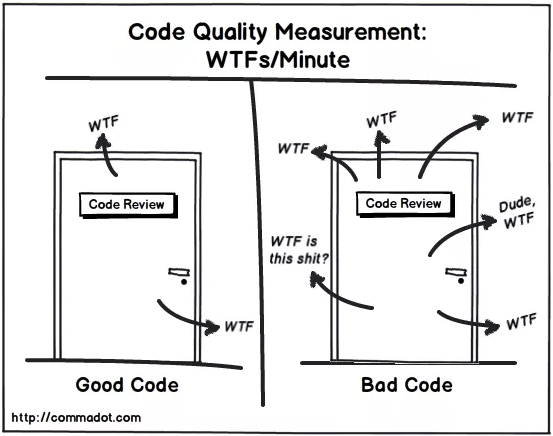
\includegraphics[width=0.7\textwidth]{wtfsMin.png}
                \end{center}
                \vspace{-0.8cm}
                \attribution{http://commadot.com, Thom Holwerda}
            \end{column}
            \begin{column}{0.5\textwidth}
                \begin{center}
                    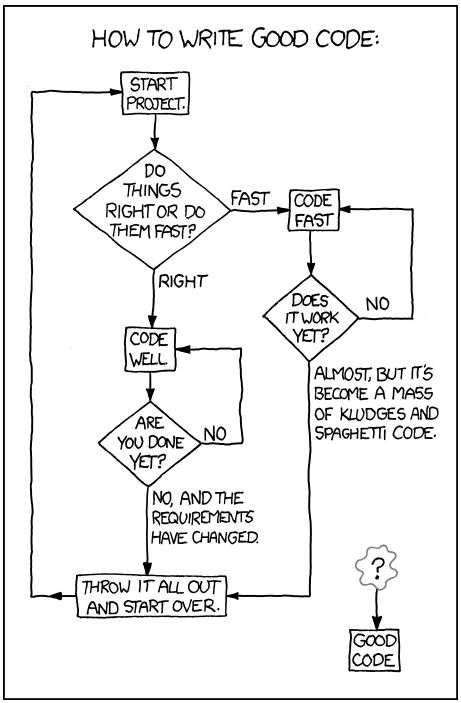
\includegraphics[width=0.7\textwidth]{goodCodeXkcd.png}
                \end{center}
                \vspace{-0.8cm}
                \attribution{https://xkcd.com}
            \end{column}
        \end{columns}
    \end{frame}

\end{document}
